\section{Introduction}
\label{sec:introduction}
Population tail-risk claims guide decisions about whether a predictor meets an acceptable loss limit and whether one predictor has lower tail risk than another. Yet historical decisions determine which outcomes are available for evaluation \citep{kleinberg2015prediction,kleinberg2018human,lakkaraju2017selective}, and the missing cases can carry the largest prediction losses. For example, a hospital assessing a model for 30-day adverse events may lack event status for patients who receive subsequent care outside its network; record linkage can later recover those labels. Conditional value-at-risk (CVaR) averages the upper tail of prediction loss \citep{acerbi2002expected,artzner1999coherent,rockafellar2000optimization}. Certifying this quantity for all target patients therefore requires an explicit account of hidden outcomes.

The obstacle persists even if the observed distribution is known exactly. Suppose labels are
observed for 25\% of a population with constant covariates, with equal proportions of zeros and ones
among observed outcomes. Under zero-one loss and CVaR at \(\alpha=.5\), the constant predictors
\(f=0\) and \(g=1\) have identical observed loss distributions. If every hidden label is zero, their
population CVaRs are \((.25,1)\); if every hidden label is one, they are \((1,.25)\). Both worlds
produce the same records and have positive observation probability. This illustration allows
unrestricted hidden outcomes and shows why historical records alone cannot certify an ordering
(Appendix~\ref{app:examples}).

We make the assumptions needed for certification explicit through a finite, externally specified
sensitivity level \(\Gamma\), which limits how much outcome odds can differ between hidden and
observed cases at the same covariates. The compatible population laws yield a sharp CVaR interval:
every value in it is attained under the observations and the restriction. Its width measures
ambiguity that persists even with unlimited historical data. Figure~\ref{fig:framework} depicts this
range for one fixed predictor; the additional enlargement accounts for estimating its endpoints from
a finite sample.

\begin{figure}[t]
\centering
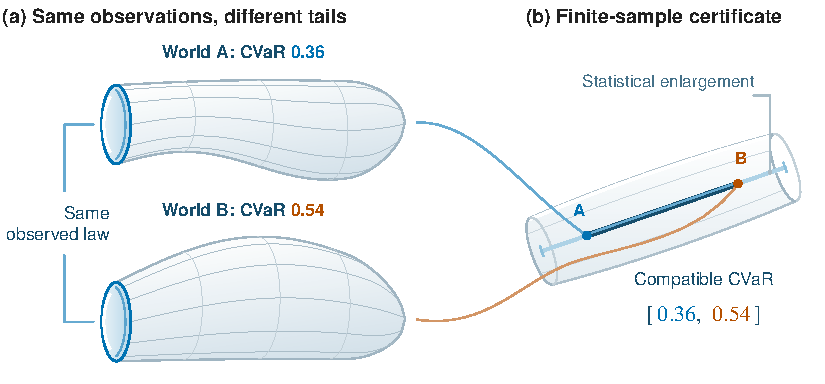
\includegraphics[width=\textwidth]{figures/fig01_concept.pdf}
\caption{\textbf{Risk ambiguity and statistical uncertainty for one fixed predictor.} (a) The same observed law is compatible with hidden-outcome laws giving population CVaR 0.36 and 0.54. (b) The dark segment is the sharp population interval; pale extensions account for estimating its endpoints from a finite sample. Colors link the laws to the endpoints. Geometry is schematic. Appendix~\ref{app:examples} gives the numerical construction.}
\label{fig:framework}
\end{figure}

Our goal is to connect three questions: which risks are compatible with the evidence, how precisely
their bounds can be estimated, and which additional labels most reduce unresolved ambiguity. An
upper bound below a chosen loss limit certifies that criterion; separated intervals establish a
predictor ordering. When these rules leave a decision unresolved, targeted outcome collection can
reduce the underlying information gap.

\paragraph{Contributions.}
\begin{enumerate}
\item \textbf{Sharp population identification.} For binary outcomes and bounded losses, we derive attainable CVaR endpoints and show that every intermediate risk is compatible. For each endpoint, one hidden-outcome law is extremal at every loss threshold, reducing its calculation to a scalar convex minimization (Section~\ref{sec:population}).

\item \textbf{Uniform finite-sample certification.} Paired, locally robust endpoint estimates give simultaneous bounds across candidate predictors at fixed sensitivity and tail levels. The bounds expose the costs of assessing a smaller tail, weaker observation overlap, and auxiliary-estimation error, and support comparisons and predictor selection using the same data (Section~\ref{sec:learning}).

\item \textbf{Minimum-cost revelation.} Under a specified information model, ranking tail identification value per unit cost gives the exact optimal revelation allocation for a fixed predictor and threshold. A zero-threshold bound also controls optimized interval width (Section~\ref{sec:revelation}).
\end{enumerate}

Revelation recovers existing outcomes for a fixed target population. Our information model treats
audited contributions as known and retains the original sensitivity bounds separately for audited
and still-hidden groups.

Synthetic experiments separate persistent identification width from decreasing endpoint error
(Figure~\ref{fig:finite-sample}). Historical LendingClub data illustrate changes in population
assessment, while controlled masking of known outcomes evaluates coverage and comparisons
(Figure~\ref{fig:lendingclub}). Fixed and sequential audits examine how acquisition choices change
estimated ambiguity (Figure~\ref{fig:revelation-results}).

\paragraph{Positioning.}
This work connects selective-label evaluation \citep{chen2025selective,coston2021fairness,lakkaraju2017selective} and partial identification \citep{manski1989anatomy,manski2003partial,scharfstein1999adjusting,tan2006distributional,zhao2019sensitivity} with CVaR optimization \citep{delage2010distributionally,duchi2021uniform,rockafellar2002conditional} and orthogonal estimation \citep{chernozhukov2018double,kallus2024localized,robins1994estimation}. Appendix~\ref{app:connections} develops these connections. We first make the target risk and the assumptions linking observed and hidden outcomes precise.
